\documentclass[10pt,twocolumn,letterpaper]{article}

\usepackage{cvpr}
\usepackage{times}
\usepackage{epsfig}
\usepackage{graphicx}
\usepackage{amsmath}
\usepackage{amssymb}
\usepackage{mathrsfs}
\usepackage{mathtools}
\usepackage{subfigure}
\DeclareMathOperator*{\argmin}{arg\,min}
% Include other packages here, before hyperref.

% If you comment hyperref and then uncomment it, you should delete
% egpaper.aux before re-running latex.  (Or just hit 'q' on the first latex
% run, let it finish, and you should be clear).
\usepackage[pagebackref=true,breaklinks=true,letterpaper=true,colorlinks,bookmarks=false]{hyperref}

\newcommand{\deva}[1]{\textcolor{red}{[Deva: #1]}}
\newcommand{\songfan}[1]{\textcolor{blue}{[Songfan: #1]}}

% \cvprfinalcopy % *** Uncomment this line for the final submission

\def\cvprPaperID{****} % *** Enter the CVPR Paper ID here
\def\httilde{\mbox{\tt\raisebox{-.5ex}{\symbol{126}}}}

% Pages are numbered in submission mode, and unnumbered in camera-ready
\ifcvprfinal\pagestyle{empty}\fi
\begin{document}

%%%%%%%%% TITLE
\title{DAG-CNNs for multi-scale recognition}

\author{First Author\\
Institution1\\
Institution1 address\\
{\tt\small firstauthor@i1.org}
% For a paper whose authors are all at the same institution,
% omit the following lines up until the closing ``}''.
% Additional authors and addresses can be added with ``\and'',
% just like the second author.
% To save space, use either the email address or home page, not both
\and
Second Author\\
Institution2\\
First line of institution2 address\\
{\tt\small secondauthor@i2.org}
}

\maketitle
%\thispagestyle{empty}

%%%%%%%%% ABSTRACT
\begin{abstract}
\deva{Need to update} \songfan{Please review this}

We present a directed-acyclic graph (DAG) deep Convolutional Neural Network (CNN) architecture. This model links various average-pooled rectified linear units (ReLU) to the final loss score layer. We demonstrate this DAG structure captures multi-scale feature for highly-variant scene classification. We also show that DAG-CNNs can be discriminatively trained in an end-to-end fashion with similar efficiency as a classical \textit{chain} model. We present extensive analysis and results on standard scene benchmarks and show state-of-the-art classification performance on all benchmarks, \ie $55.5\%$ on SUN397, $76.1\%$ on MIT67, and $92.4\%$ on Scene15.

\end{abstract}

%%%%%%%%% BODY TEXT
\section{Introduction}


\begin{figure}[t!]
\centering
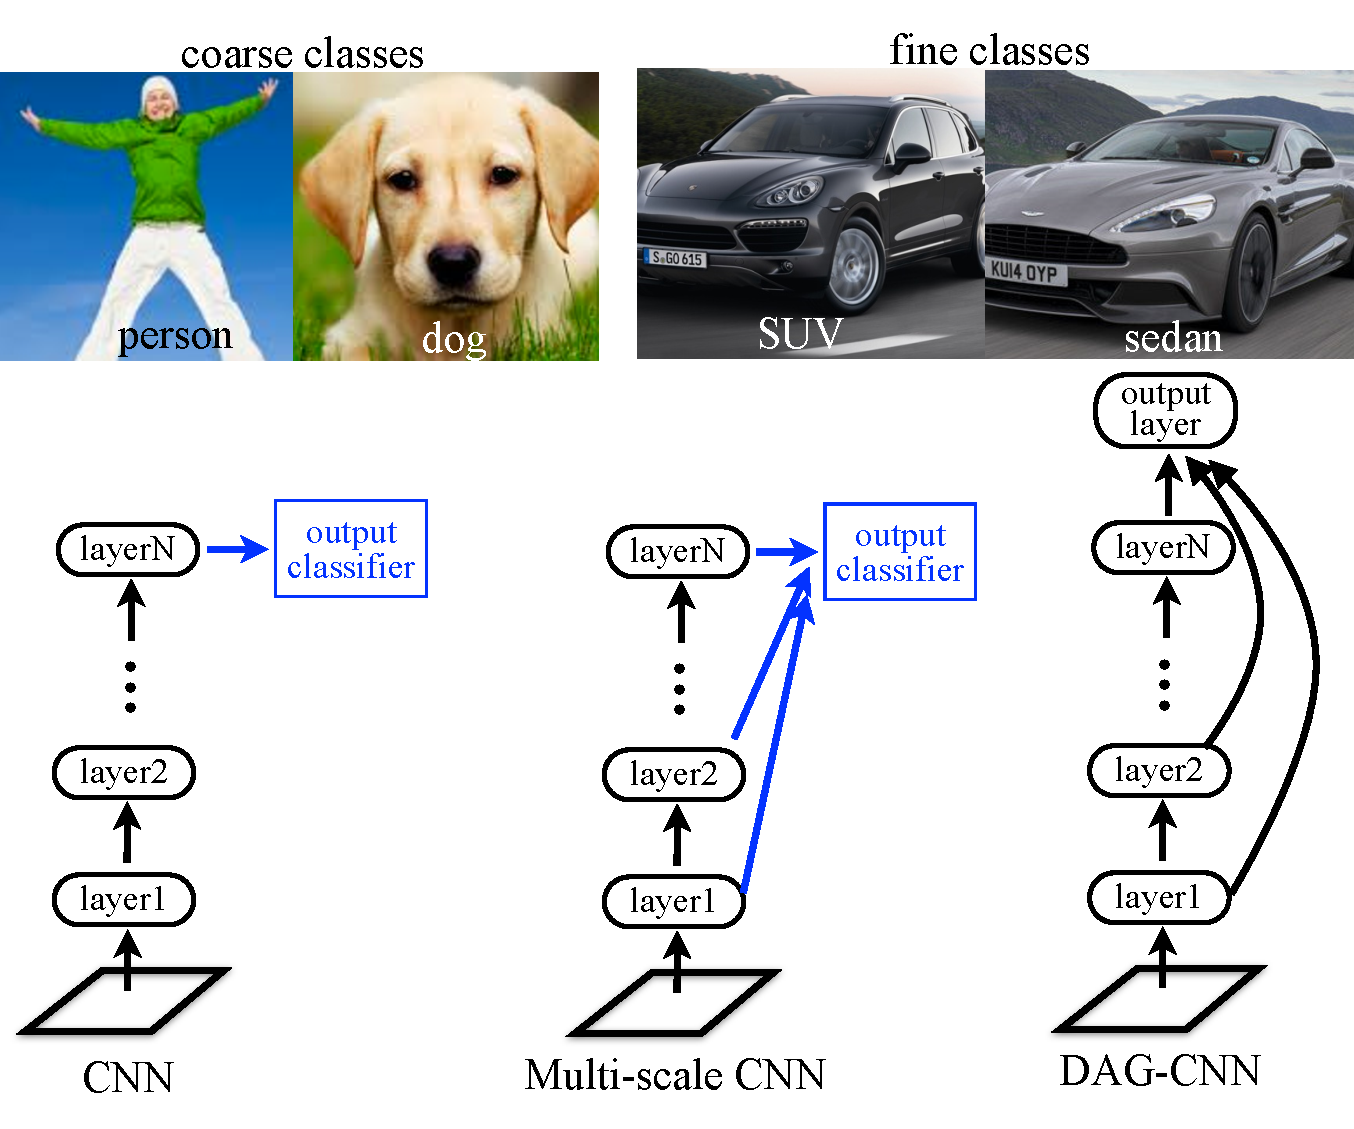
\includegraphics[width=\columnwidth]{fig/deva_splash}
\caption{Recognition typically require features at multiple scales. Distinguishing a person versus dog requires highly invariant features robust to the deformation of each category. On the other hand, fine-grained recognition likely requires detailed shape cues to distinguish models of cars ({\bf top}). We use these observations to revisit deep convolutional neural net (CNN) architectures. Typical approaches train a classifier using features from a single output layer ({\bf left}). We extract multi-scale features from multiple layers to simultaneously distinguish coarse and fine classes. Such features come ``for free'' since they are already computed during the feed-forward pass ({\bf middle}). Interestingly, the entire multi-scale predictor is still a feed-forward architecture that is no longer chain-structured, but a directed-acyclic graph (DAG) ({\bf right}). We show that DAG-CNNs can be discriminatively trained in an end-to-end fashion, yielding state-of-the-art recognition results across various recognition benchmarks.  DAG-CNNs address some well-known challenges with CNNs such as ``vanishing gradients''~\cite{bengio1994learning}. Lower layers in a DAG-CNN still receive a strong gradient signal during learning because they are directly tied to the output layer, making them easier to train.
\label{fig:splash}}
\end{figure}

Deep convolutional neural nets (CNNs), pioneered by Lecun and collaborators~\cite{lecun1998gradient}, now produce state-of-the-art performance on many visual recognition tasks~\cite{AlexNet, overfeat, veryDeep, GoogLeNet, nin}. An attractive property is that appear to serve as universal feature extractors, either as ``off-the-shelf'' features or through a small amount of ``fine tuning''. CNNs trained on particular tasks such as large-scale image classification~\cite{ImageNet} {\em transfer} extraordinarily well to other tasks such as object detection~\cite{rcnn}, scene recognition~\cite{zhoulearning}, image retrieval~\cite{Gong14}, etc \cite{cnn_baseline}.

{\bf Hierarhical chain models:}  CNNs are 
hierarchical feed-forward architectures that compute progressively invariant representations of the input image. However, the appropriate level of invariance might be task-dependent. Distinguishing people and dogs requires a representation that is robust to large spatial deformations, since people and dogs can articulate. However, fine-grained categorization of car models (or bird species) requires fine-scale features that capture subtle shape cues. We argue that a universal architecture capable of both tasks must employ some form of multi-scale features for output prediction.

\begin{figure*}
\centering
	\subfigure[mid-level feature is preferred]{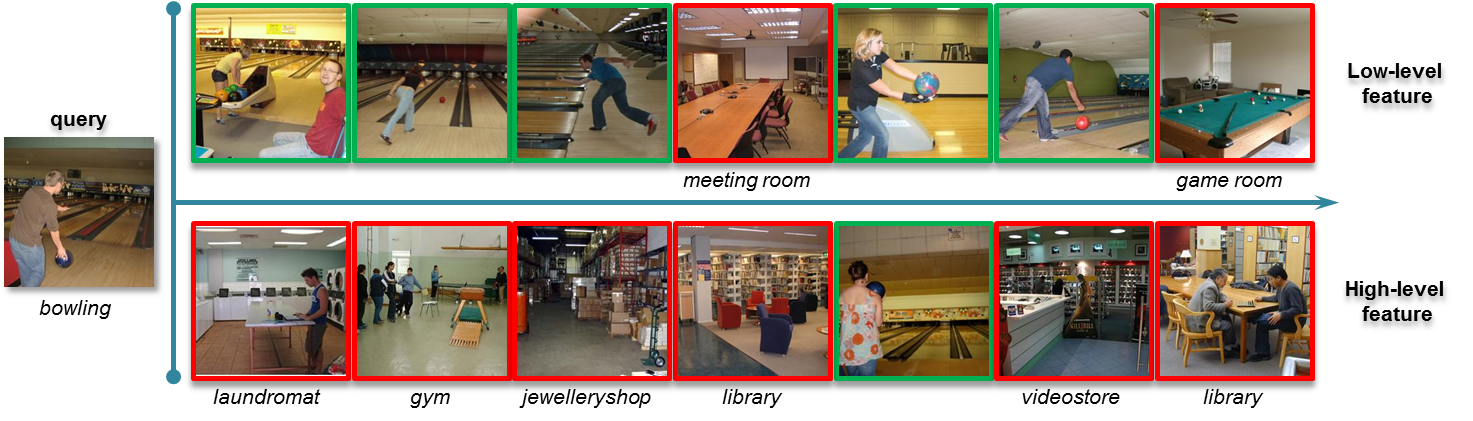
\includegraphics[width=.9\textwidth]{fig/moti_low_better.png}\label{fig:moti_low}}
	\subfigure[high-level feature is preferred]{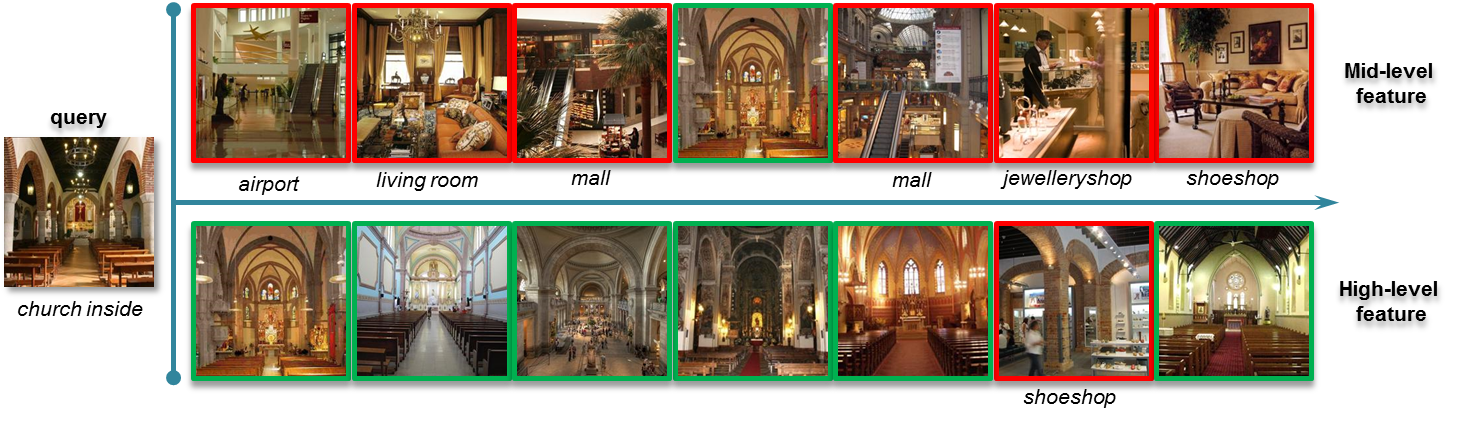
\includegraphics[width=.9\textwidth]{fig/moti_high_better.png}\label{fig:moti_high}}

\caption{Retrieval results using L2 distance for both mid- and high-level features on MIT67~\cite{MIT67}, computed from layer 11 and 20 of the Caffe model. \textit{Green} (\textit{Red}) box means correct (wrong) results, in terms of the scene category label. The correct label for wrong retrievals are provided. The retrieval results are displayed such that the left-most image has the closest distance to the query, and vice versa. Certain query images (or categories) produce better matches with high-level features, while others produce better results with mid-level features. This motivates our multi-scale approach. \deva{Replace bolwing with florist or greenhouse image, more consistent with per-class plots.}\songfan{Done. BTW, I intentional leave all your question intact so that you can see all the concern you have is been addressed or not. Does this make sense? Or do you want me to just delete the our in-latex conversation after the question is been addressed?}}
\label{fig:moti}
\end{figure*}


{\bf Multi-scale features:} We introduce multi-scale CNN architectures that use features at multiple scales for output prediction (Fig.~\ref{fig:splash}). From one perspective, our architectures are quite simple. Typical approaches train a output predictor (e.g., a linear SVM) using features extracted from a single output layer. Instead, one can train an output predictor using features extracted from multiple layers. Note that these features come ``for free''; they are already computed in a standard feed-forward pass. 

{\bf Marginal activations:} One difficulty with multi-scale approaches is feature dimensionality - the total number of features across all layers can easily reach hundred of thousands. This makes training even linear models difficult and prone to overfitting. Instead, we use marginal activations computed from sum (or max) pooling across all spatial locations in a given activation layer. From this perspective, our models are similar to those that compute multi-scale features with spatial pooling, including multi-scale templates~\cite{felzenszwalb2008discriminatively}, orderless models\cite{Gong14}, spatial pyramids~\cite{spatial_pyramid}, and bag-of-words~\cite{sivic2003video}.

{\bf DAG-CNN:} Our multi-scale model differs from such past work in one notable aspect. Our model is still a feed-forward CNN that is no longer chain-structured, but a directed-acyclic graph (DAG). DAG-structured CNNs can be discriminatively trained in an end-to-end fashion, allowing us to learn multiscale representations. Multi-scale learning addresses one well-known difficulty of CNNs - the ``vanishing gradient'' problem~\cite{bengio1994learning}. During gradient-based learning, the gradient signal becomes progressively diluted as one back-propogates it through multiple layers, such that the bottom-most layer receives essentially no updates. Our multi-scale DAG structure connects all activation layers directly to the output, ensuring they all receive a strong gradient signal during learning. 

%yeilding state-of-the-art recognition results across various recognition benchmarks. 

% Trained with large number of instances, (such as ImageNet~\cite{ImageNet}), CNN is also an excel candidate for off-the-shelf feature extractions, results in outstanding performance in various recognition tasks~\cite{cnn_baseline}. In the meantime, a considerable amount of effort is spent on how to further improve the performance of CNN. On one hand, many are focus on techniques to efficiently and effective train a CNN. A good initialization need to be carefully selected~\cite{diff_cnn} in the beginning. Data augmentation~\cite{AlexNet} is recommended to improve the model performance as well. Drop-out~\cite{dropout} and momentum~\cite{momentum} are also necessary to prevent over-fitting and obtain superior models. On the other hand, different model components and architectures are proposed. Rectified linear units (ReLU)~\cite{AlexNet} add non-linearity and enrich the model complexity. Different pooling method, such as Distance Transform Pooling~\cite{dist_trans}, is adopted in~\cite{dpm_is_cnn}, allowing local deformations, as in the widely-used deformable part-based model (DPM)~\cite{dpm}. \cite{veryDeep} adopts a small $3\times 3$ receptive field to deepen the model, while maintaining less parameters. A network in network~\cite{nin} is proposed to enhance model discriminability for local patches within the receptive field. The award winning GoogLeNet~\cite{GoogLeNet} uses an \textit{Inception} model that is based on the Hebbian principle~\cite{Hebb}, \ie, neurons that fire together, wire together, the theoretical proof of which is provided by~\cite{dnn_proof} under constraints. 

%One question to ponder: is there any model-independent potential that is yet to be discovered. Although allowing local deformation, CNN encodes the the spatial information of multi-scale features. Conversely, by ignoring the spatial location of features, bag-of-feature like techniques~\cite{spatial_pyramid} achieves transformation invariance to some extend. As pointed out in~\cite{Gong14}, combining both type of features results in a better representation for recognition tasks with large variations, such as Scene classification~\cite{SUN397,MIT67}. Traditionally, when CNN is used for feature extraction, the activation of the first fully-connected (FC) layer is usually considered as the feature~\cite{overfeat, Gong14}. Using an off-the-shelf deep CNN model,~\cite{Gong14} explicitly extracts image patches from three scales and computes the feed-forward CNN activations for each patch for feature extraction. This algorithm is cumbersome due to the computation of multiple patches for one image. Besides, it can only encode the multi-scale features to a certain extend limited by the burden of the post processing, \ie, K-means and Principle Component Analysis (PCA). As a matter of fact, CNN feature is meant to encode multi-scale feature at each convolutional (Conv.) layer. Therefore, there is no need to extract multi-scale patches and only one feed-forward computation is sufficient to capture the activations of multi-scale features for one input image. 


%In this paper, we first conducted an empirical analysis on the feature discriminativeness of every unit of CNN model. By average-pooling at each layer, the output ignores global spatial information and results in a bag-of-feature representation. The bag-of-feature from ReLU is then found to carry the most performance gain at each layer. We have also observed a synergy of multi-scale activations results in a better discriminative representation. These observations tie closely to the vanishing gradient~\cite{diff_cnn} issue in the deep CNN literature. During the training of a CNN, the top layer can be easily saturated. The gradients in the back-propagation algorithm will not effective reach the lower levels, resulting in a model that focuses more high-level features. Thus, we proposed a model augmentation schema, BoMSA, that chains the ReLU at each layer to the ultimate loss function. This augmentation approach is not confined by model variations and can be applied to existing pre-trained models or re-training the model from the ground up. By explicitly linking the lower layers to the decision layer, we gear the training towards the bag-of-activations from all layers. Thus, the augmented model is designed to be robust to spatial translations while maintaining its discriminative power in the multi-scale fashion.

{\bf DAG-structured Neural Networks:} DAG-structured neural nets have been previously explored in the context of recurrent neural nets \cite{baldi2003principled,graves2009offline}. Recurrent neural nets use feedback to capture dynamic states, and so typically cannot be processed with feedforward computations. Previous work has also shown that long-range connections between neural layers can eliminate the vanshing gradient problem, but this is done in the context of memory-based networks~\cite{hochreiter1997long}. We make use of DAG structures to efficiently encode multi-scale features in a simpler feed-forward network.

{\bf Overview:} We motivate our multi-scale DAG-CNN model in Sec.~\ref{sec:motivation}, describe the full architecture in Sec.~\ref{sec:ana}, and conclude with numerous benchmark results in Sec.~\ref{sec:exp}. We evaluate multi-scale DAG-structured variants of existing CNN architectures (\eg, Caffe~\cite{Caffe}, Deep19~\cite{veryDeep}) on a variety of scene recognition benchmarks including SUN397~\cite{SUN397}, MIT67~\cite{MIT67}, Scene15~\cite{Scene15}. We observe a consistent improvement regardless of the underlying CNN architecture, producing state-of-the-art results on all 3 datasets.

%A consistent performance improvement is observed of our multi-scale representation over the best discriminative single-scale feature. 
%The rest of the paper is organized as follows: we motivate and describe our model augmentation approach in Sec.~
%\ref{sec:approach}. An in-depth analysis is provided in Sec.~\ref{sec:ana}. Systematic experimental results are included in Sec.~\ref{sec:exp}. 


%-------------------------------------------------------------------------
%-------------------------------------------------------------------------
\section{Motivation\label{sec:motivation}}

In this section, we motivate our multi-scale architecture with a series of empirical analysis. We carry out an analysis on existing CNN architectures, namely Caffe and Deep19. Caffe~\cite{Caffe} is a broadly used CNN toolbox. It includes a pre-trained model ``AlexNet''~\cite{AlexNet} model, learned with millions of images from the ImageNet dataset~\cite{ImageNet}. This model has 6 conv. layers and 2 fully-connected (FC) layers. Deep19~\cite{veryDeep} uses very small $3\times 3$ receptive fields, but an increased number of layers -- 19 layers (16 conv. and 3 FC layers). This model produced state-of-the-art performance in ILSVRC-2014 classification challenge~\cite{ILSVRC14}. We evaluate both models on the heavily benchmarked MIT Indoor Scene (MIT67) dataset~\cite{MIT67}, using 10-fold cross-validation.

\subsection{Single-scale models} 
%We first verify our hypothesis that different recognition tasks require different amounts of invariance through two experiments.

{\bf Image retrieval:} Recent work that explores sparse reconstruction techniques for visualizing and analyzing features~\cite{vondrick2013hoggles}. Inspired by such techniques, we use image retrieval to begin our exploration. We attempt to ``reconstruct'' a query image by finding $N=5$ closest images in terms of L2-distance, when computed with mean-pooled layer-specific activations. Results are shown for two query images and two Caffe layers in Fig.~\ref{fig:moti}. The {\tt florist} query image tends to produces better matches when using mid-level features that appear to capture \textit{objects} and \textit{parts}. On the other hand, the {\tt indoor-church} query image tends to produce better matches when using high-level features that appear to capture more global \textit{scene} statistics.


%By working with poo providing some degree of robustness to spatial transformation of objects (bowling ball and people body parts). On the other hand, the example in Fig.~\ref{fig:moti_high} shows high-level feature captures the spatial geometry information. This is important for classes such as scenes with strong \textit{structure} cues, \eg, church, cloister, corridor, etc. Thus, we wish to develop a method that captures the multi-scale invariance.



%\subsection{Scale-specific classification}
%We carry out an analysis on existing CNN architectures, namely Caffe and Deep19. Caffe~\cite{Caffe} is a broadly used CNN toolbox. It includes a pre-trained model ``AlexNet''~\cite{AlexNet} model, learned with millions of images from the ImageNet dataset~\cite{ImageNet}. This model has 6 conv. layers and 2 fully-connected (FC) layers. Deep19~\cite{veryDeep} uses very small $3\times 3$ receptive fields, but an increased number of layers -- 19 layers (16 conv. and 3 FC layers). This model produced state-of-the-art performance in ILSVRC-2014 classification challenge~\cite{ILSVRC14}. We evaluate both models on the heavily benchmarked MIT Indoor Scene (MIT67) dataset~\cite{MIT67}.

\begin{figure}[htbp]
\centering
	\subfigure[Caffe]{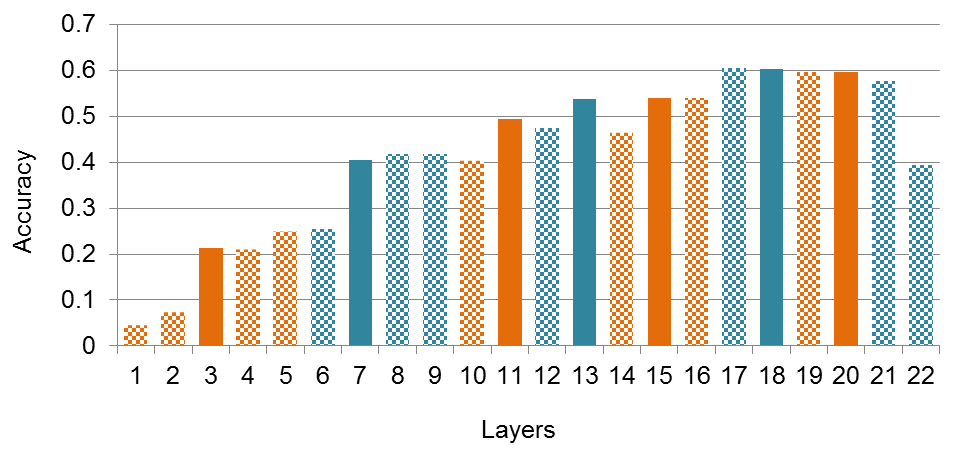
\includegraphics[width=\columnwidth]{fig/fig_layer_caffe.png}\label{fig:layer_caffe}}
	\subfigure[Deep19]{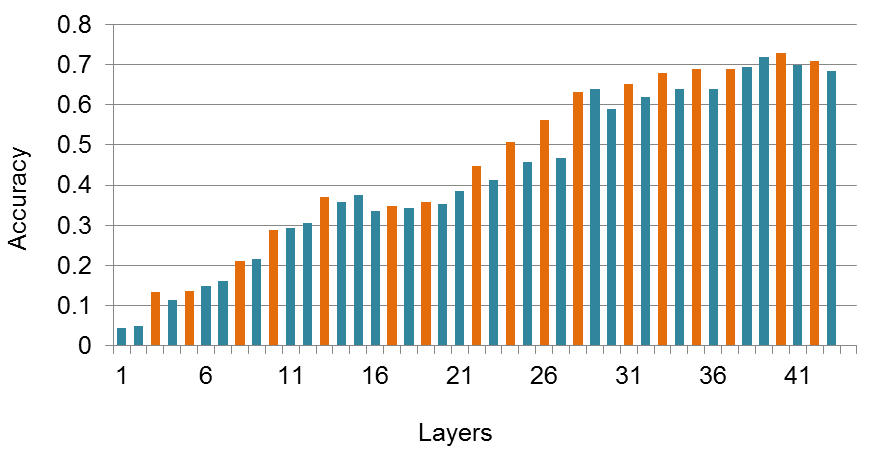
\includegraphics[width=\columnwidth]{fig/fig_layer_deep19.png}\label{fig:layer_deep19}}
\caption{The classification accuracy on MIT67~\cite{MIT67} using activations from each layer. We use a solid color fill representing the output of a ReLU layer. There are 7 ReLU layers for the Caffe model and 18 for Deep19. We see tend to see a performance jump at each successive RelU layer, particularly earlier on in the model.}
\label{fig:layer_MIT67}
\end{figure}

{\bf Single-scale classification:} Following past work \cite{cnn_baseline}, we train a linear SVM classifier using features extracted from a particular layer. We specifically train $K=67$ 1-vs-all linear classifiers.
We plot the performance of single-layer classifiers in~\ref{fig:layer_MIT67}. The detailed parameter options for both Caffe and Deep19 models are described later in Sec.~\ref{sec:exp}. As past work has pointed out, we see a general increase in performance as we use higher-level (more invariant) features. We do see a slight improvement at each nonlinear activation (ReLU) layer. This makes sense as this layer introduces a nonlinear rectification operation $\max(0,x)$, while other layers (such an convolutional or sum-pooling) are linear operations that can be learned by a linear predictor.



\begin{figure*}[ht!]
\centering
	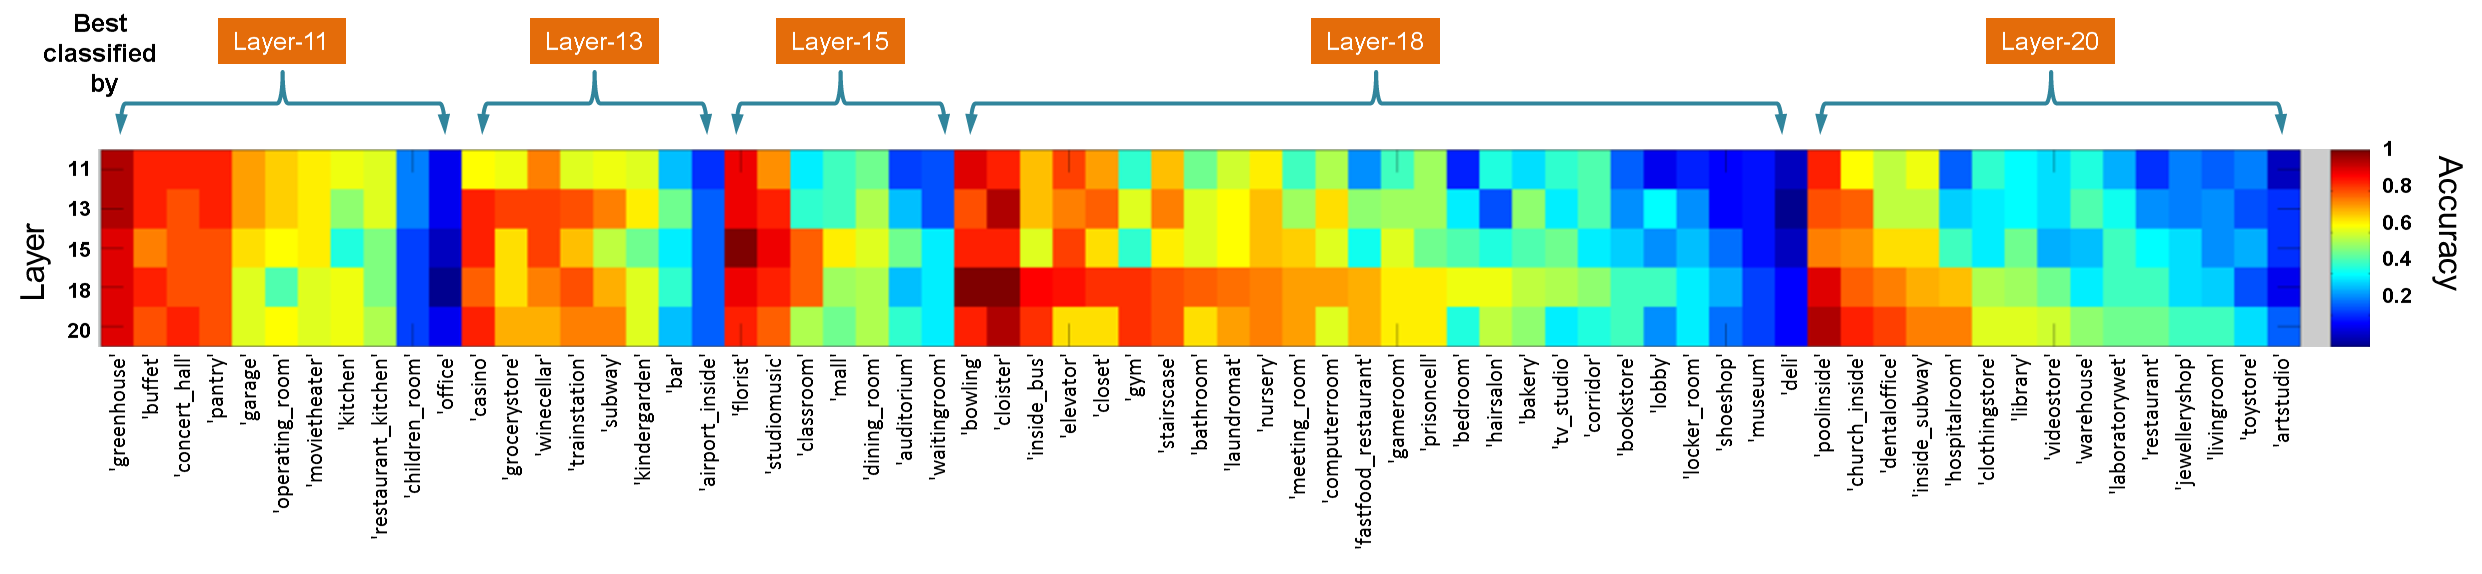
\includegraphics[width=1\textwidth]{fig/fig_level_perf.png}
\caption{The ``per-class'' performance using various levels of feature. \deva{Re-order into the 5 groups from Fig.4 [histogram of best-performing layer]. Hopefully these groups will be visually apparent!} 
\songfan{Done}}
\label{fig:level_perf}
\end{figure*}


{\bf Scale-varying classification:} The above experiment required training $K \times N$ 1-vs-all classifiers, where $K$ is the number of classes and $N$ is the number of layers. We can treat each of the $KN$ classifiers as binary predictors, and score each with the number of correct detections of its target class. We plot these scores as a matrix in Fig.~\ref{fig:level_perf}. We tend to see groups of classes that operate best with features computed from particular high-level or mid-level layers. Indeed, we plot the optimal scale for each binary predictor in Fig.~\ref{fig:best_perf_layer_hist}. Most categories tend to do well with high-level features, but a significant fraction (over a third) do better with mid-level features.

\begin{figure}[htbp]
\centering
	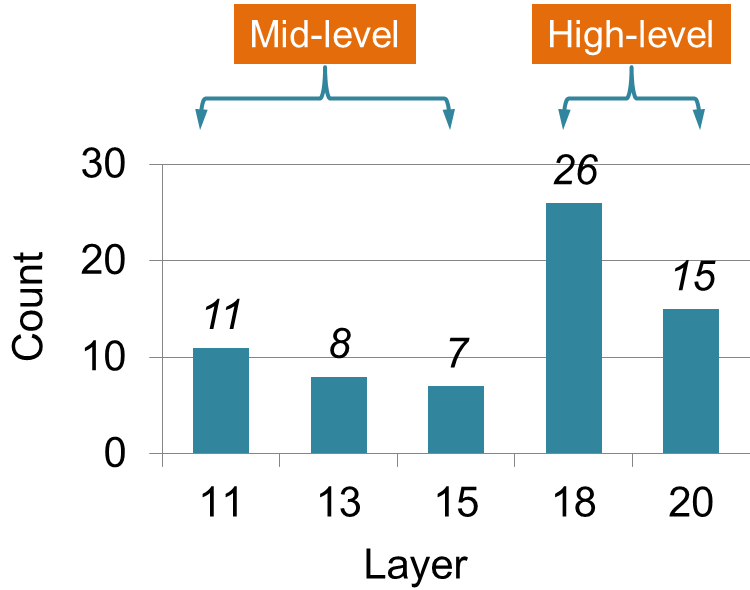
\includegraphics[width=.6\columnwidth]{fig/best_perf_layer_hist.png}
\caption{The class histogram of best-performing layer. The high-level feature, extracted from Layer-18,  has the best discriminativeness among all selected layers, achieving the highest accuracy in the 26 categories. In the meantime, mid-level features (Layer-11,13, and 15) are also important in this classification task. They perform the best for another 26 categories. }
\label{fig:best_perf_layer_hist}
\end{figure}

\subsection{Multi-scale models} 
{\bf Multi-scale classification:} We now explore the use of multi-scale features. One immediate hurdle to including all features from all layers is the massive increase in dimensionality. As such, we compute only marginal activations at each RelU layer with average pooling. We found average pooling to outperform sum pooling as the resulting marginal features remained in a reasonable dynamic range. We also experimented with max-pooling, but found similar performance. Specifically, assume a particular layer is of size $H \times W \times F$, where $H$ is the height, $W$ is the width, and $F$ is the number of filter channels. We compute a $1 \times 1 \times F$ feature by averaging across spatial dimensions. Note that the ``marginal activations'' of fully-connected layers (which are already of dimension $H \times 1 \times F$) are simply the original activations. We plot performance as we iteratively add more layers. Fig.~\ref{fig:layer_MIT67} suggests that the last RelU layer is a good strarting point due to its strong single-scale performance. Fig~\ref{fig:add_back} plots performance as we add previous layers to the classifier feature set. Performance increases as we add intermediate layers, while lower layers prove less helpful (and may even hurt performance, likely do to overfitting). Our observations suggest that high and mid-level features (\ie, \textit{parts} and \textit{objects}) are more useful than low-features based on \textit{edges} or \textit{textures} in scene classification. 


% the performance increase in the beginning by adding mid-level features to enrich the model discriminativeness. However, including some low level responses to the feature actually hurts the performance, \ie, layer 7 and 3 in Fig.~\ref{fig:add_back_caffe}. 

%Since different CNN layers correspond to image feature at various scales, seen in Fig.~\ref{fig:moti}, we wonder whether combining activations at multiple scales help to extract a better feature. To address this question, we carried out another experiments on the MIT67 data~\cite{MIT67}. We start from the average-pooled response of the last ReLU layer and greedily concatenate the ones from previous ReLU layers. The reason we start from the last ReLU layer is that, in the literature when CNN is used for feature extraction, the response of the first fully connected layer is usually selected~\cite{cnn_baseline,Gong14}. Besides, our previous analysis in Fig.~\ref{fig:layer_MIT67} also demonstrates better discriminative power of high-level CNN layer.

%The rest of the experimental setups are the same as in Sec.~\ref{sec:indi_scale}, \ie, a set of 67-way one-vs-all linear SVM classifiers are trained every time we add one more layer. Since we keep on concatenating features at lower level, the feature dimension is monotonically increasing. As the results shown in Fig.~\ref{fig:add_back}, the performance increase in the beginning by adding mid-level features to enrich the model discriminativeness. However, including some low level responses to the feature actually hurts the performance, \ie, layer 7 and 3 in Fig.~\ref{fig:add_back_caffe}. We believe it demonstrates the benefit of incorporating more discriminative mid-level and high-level features of CNN (\ie, \textit{parts} and \textit{objects}), but not necessarily the low-level features, such as \textit{edge} or \textit{textures}. 

\begin{figure}[htbp]
\centering
	\subfigure[Caffe]{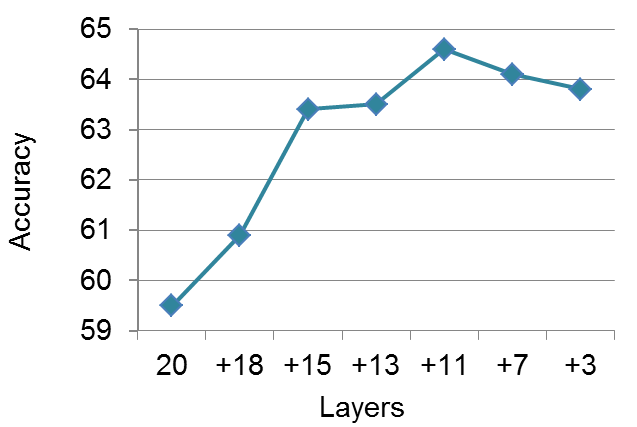
\includegraphics[width=.43\columnwidth]{fig/fig_add_back_caffe.png}\label{fig:add_back_caffe}}
	\subfigure[Deep19]{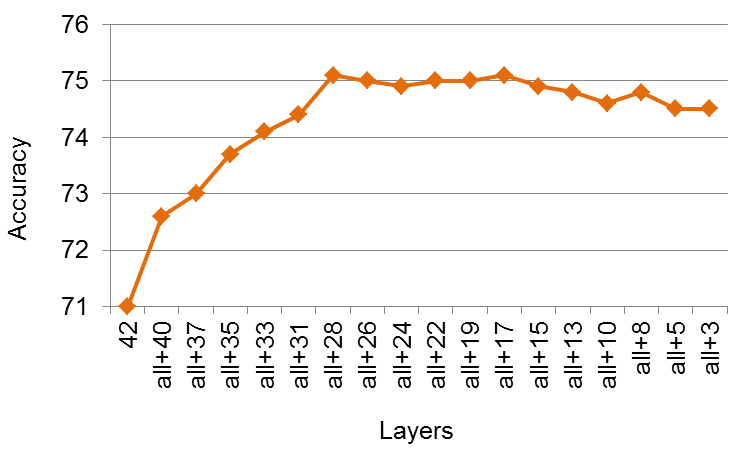
\includegraphics[width=.56\columnwidth]{fig/fig_add_back_deep19.png}\label{fig:add_back_deep19}}
\caption{We plot performance of a multi-scale classifier as we add more layer-specific features. We start with the last RelU layer, and iteratively add the previous RelU layer to the feature set of the classifier.
The ``+'' sign the recent-most added layer. Adding additional layers help, but performance saturates and even slightly decreases when adding lower-layer features. This suggests it may be helpful to search for the ``optimal'' combination of layers.}
\label{fig:add_back}
\end{figure}

{\bf Multi-scale selection:} The previous results show that adding all layers may actually hurt performance. We verified that this was an overfitting phenomena; additional layers always improved training performance, but could decrease test performance due to overfitting. This appears especially true for multi-scale analysis, where nearby layers may encoded redundant or correlated information (that is susceptible to overfitting). Ideally, we would like to search for the ``optimal'' combination of RelU layers that maximize performance on validation data. Since there exists an exponential number of combinations ($2^N$ for $N$ RelU layers), we find an approximate solution with a greedy forward-selection strategy. We greedily select the next-best layer (among all remaining layers) to add, until we observe no further performance improvement. As seen in Fig.~\ref{fig:forward_select_caffe}, the optimal results of this greedy approach rejects the low-level features. This is congruent with the previous results in Fig.~\ref{fig:add_back_caffe}. Similarly for the Deep19 model in Fig.~\ref{fig:forward_select_deep19}, although the feature pool is large (18 ReLU layers), the optimal greedy results includes only the mid- or high-level features. 

\begin{figure}[htbp]
\centering
	\subfigure[Caffe]{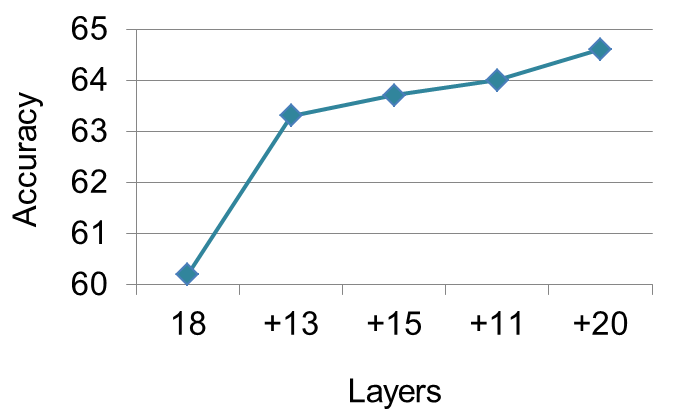
\includegraphics[width=.49\columnwidth]{fig/fig_forward_select_caffe.png}\label{fig:forward_select_caffe}}
	\subfigure[Deep19]{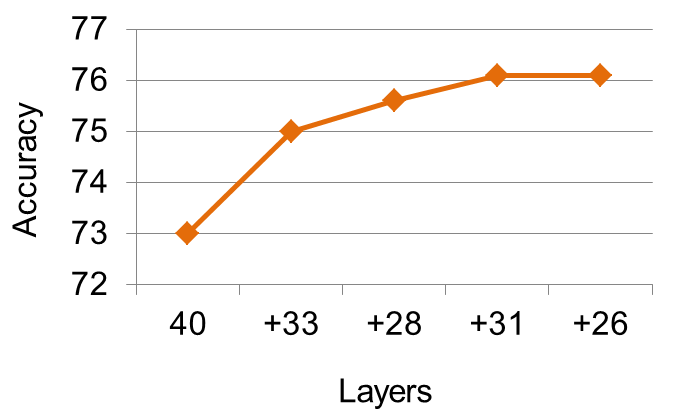
\includegraphics[width=.49\columnwidth]{fig/fig_forward_select_deep19.png}\label{fig:forward_select_deep19}}
\caption{The performance trend when using forward selection to incorporate the ReLU layers. Note that layers are {\em not} selected in high-to-low order. For example, both models begin with the second-to-last RelU layer, and skip one or more previous layers when adding the next layer. This suggests that layers encode some redundant or correlated information. Overall though, we see significant improvements of 3-5\% for both models. These results suggest that an ``off-the-shelf'' multi-scale model is already quite effective. We will show that ``fine-tuning'' with gradient-based DAG-CNN learning further improves results. Our performance increase comes with virtually no run-time cost, as these multi-scale features are already computed ``for free''.}

\label{fig:forward_select}
\end{figure}


Our analysis strongly suggest the importance (and ease) of incorporating multi-scale features for classification tasks. For our subsequent experiments, we use scales selected by the forward selection algorithm on MIT67 data (shown in Fig.~\ref{fig:forward_select}). Note that we use them for all our experimental benchmarks, demonstrating a degree of cross-dataset generatlization in our approach.

\section{Approach} 

In this section, we show that the multi-scale model examined in Fig.~\ref{fig:forward_select} can be written as a DAG-structured, feed-forward CNN. We also demonstrate that it can be trained with gradient-based learning. Essentially, one can use standard calculus constructions -- specifically the chain rule and partial derivatives -- to generalize backpropogation to layers that have multiple ``parents'' or inputs.

{\bf Model:} The run-time behaviour of our multi-scale predictor from the previous section is equivalent to feedforward processing of the DAG-strutured architecture in Fig.~\ref{fig:forward_select}. Note that we have swapped out a margin-based hinge-loss (corresponding to a SVM) with a softmax function, as the latter is more amenable to training with current toolboxes. Specifically, typical CNNS are grouped into collections of four layers, \ie, Conv., ReLU, contrast normalization (Norm), pooling layers (with the Norm and pooling layers being optional). The final layer is usually a $K$-way softmax function that predicts one of $K$ outputs. We visualize these layers as a chain-structured ``backbone''. Our DAG-CNN simply links each RelU layer to an average-pooling layer, which feeds to a fully-connected (FC) layer that produces $K$ outputs (represented formally as a $1 \times 1 \times K$ matrix) These outputs are element-wise added together across all layers, and the resulting $K$ numbers are fed into the final soft-max function. The weights of the FC layers are equivalent to the weights of the final multi-scale $K-way$ predictor (which is a softmax predictor for a softmax loss output, and a SVM for a hinge-loss output). Note that all the required operations are standard modules except for the \textit{Add}.

%modifications require standard layers, except for the \textid{Add}. Crucially, it breaks the chain-structure of the 


%Before connecting into the Soft-max layer, an \textit{Add} layer is introduced to combine the responses from all FC layers. 

\begin{figure*}[t!]
\centering
	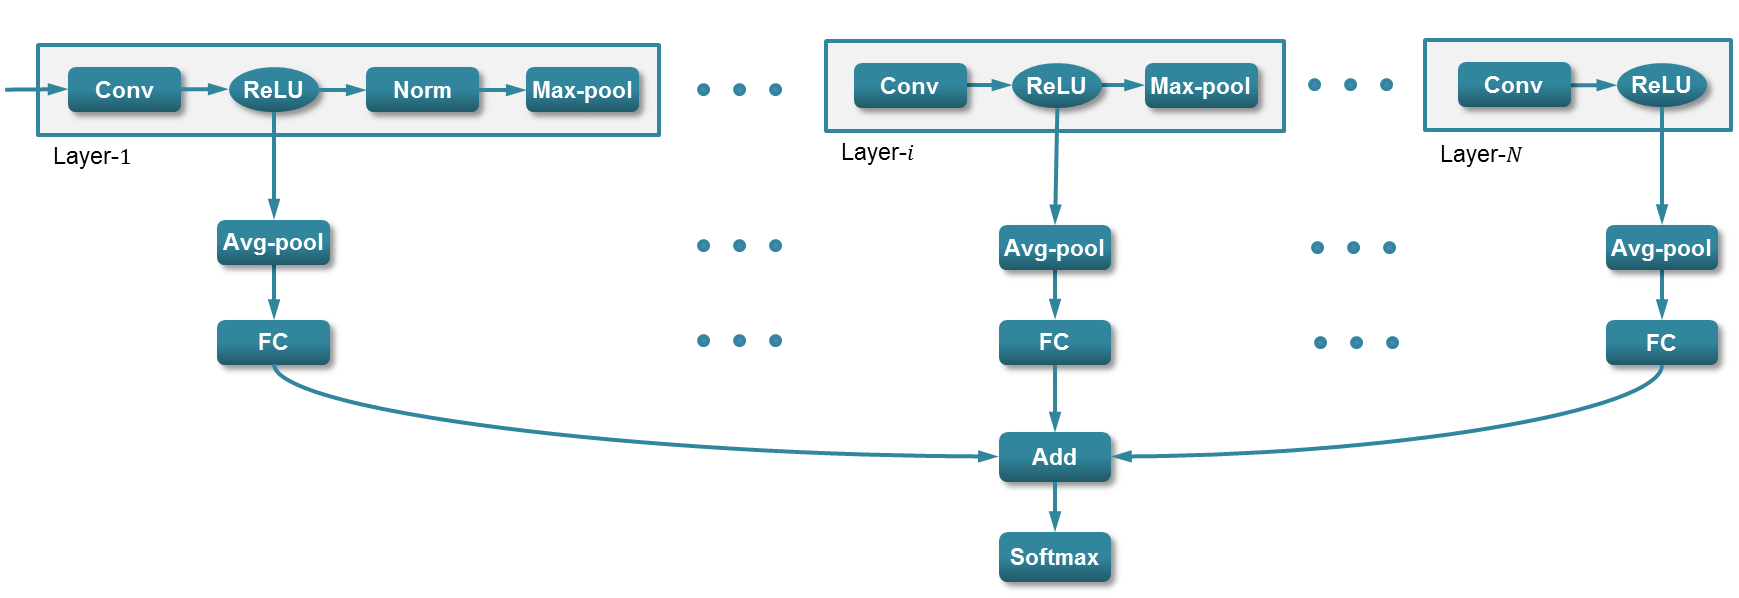
\includegraphics[width=\textwidth]{fig/fig_model.png}
\caption{Our multi-scale DAG-CNN architecture is constructed by adding (marginalized) multi-scale output connections to an underlying {\em chain backbone} from the original CNN.}
\label{fig:model}
\end{figure*}

{\bf Training:} Let $\textbf{w}_1,...\textbf{w}_K$ be the CNN model parameters at $1,..,K$-th layer, training data be ($\textbf{x}^{(i)},\textbf{y}^{(i)}$), where $\textbf{x}^{(i)}$ is the $i$-th input image and $\textbf{y}^{(i)}$ is the indicator vector of the class of $\textbf{x}^{(i)}$. Then we intend to solve the following optimization problem

\begin{align}
\argmin_{\textbf{w}_1,...\textbf{w}_K} \frac{1}{n}\sum_{i=1}^{n} \mathcal{L}(f(\textbf{x}^{(i)};\textbf{w}_1,...,\textbf{w}_K),\textbf{y}^{(i)})
\end{align}

As is now commonplace, we make use of stochastic gradient descent to minimize the objective function. For a traditional \textit{chain} model, the partial derivative of the output with respect to any one weight can be recursively computed by the chain rule, as described in the backprop algorithm~\cite{rumelhart1988learning}. 

{\bf Multi-output layers (RelU):} Our DAG-model is structurally different at the RelU layers (since they have multiple outputs) and the Add layer (since it has multiple inputs). We can still compute partial derivates by recursively applying the chain rule, but care needs to be taken at these points. Let us consider the $i$-th ReLU layer in Fig.~\ref{fig:backprop_eq}. Let $\alpha_i$ be its input, $\beta_i^{(j)}$ be the output for its $j$-th output branch (its $j^{th}$ child in the DAG), and let $z$ is the final output of the Softmax layer. The gradient of $z$ with respect to the input of the $i$-th ReLU layer can be computed as

\begin{align}
\frac{\partial z}{\partial \alpha_i}=\sum_{j=1}^{C}\frac{\partial z}{\partial \beta_i^{(j)}}\frac{\partial \beta_i^{(j)}}{\partial \alpha_i} \quad \text {(in general)} \label{eq:backprop1}
\end{align}

\noindent where $C=2$ for the example in Fig.~\ref{fig:backprop_eq}. One can recover standard backpropogation equations from the above by setting $C$=1: a single back-prop signal $\frac{\partial z}{\partial \beta_i^{(1)}}$  arrives at RelU unit $i$, is multipled by the local gradient $\frac{\partial \beta_i^{(1)}}{\partial \alpha_i^{(1)}}$, and is passed on down to the next layer below. In our DAG, {\em multiple} backprop signals arrive $\frac{\partial z}{\partial \beta_i^{(j)}}$ from each branch $j$, each is multipled by an branch-specific gradient $\frac{\partial \beta_i^{(j)}}{\partial \alpha_i}$, and their total sum is passed on down to the next layer.

% Each partial derivative component, $\frac{\partial z}{\partial \beta_i^{(j)}}\frac{\partial \beta_i^{(j)}}{\partial \alpha_i}$, can be computed in the typical back-prop fashion. In chain-structured back-propogration, a single back-prop signal \frac{\partial z}{\partial \beta_i} will arrive at RelU unit $i$. This is multiped by the layer-specific gradient $
%This means that during gradient updating, multiple $(C)$ backprop signals will arrive at the $i^{th}$ RelU layer. These signals are added together, and then 

\begin{figure}[htbp]
\centering
	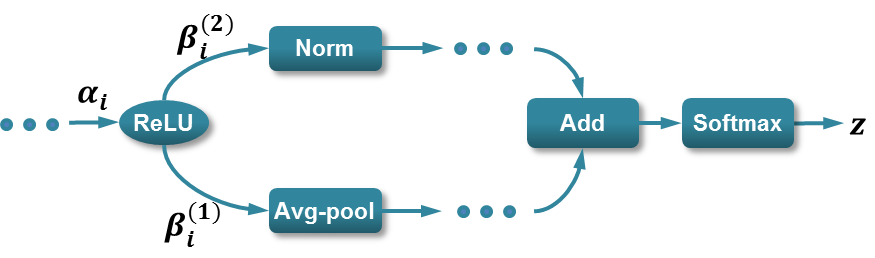
\includegraphics[width=\columnwidth]{fig/fig_backprop_eq.png}
\caption{Visualization of the parameter setup at $i$-th ReLU.}

\label{fig:backprop_eq}
\end{figure}

%Even though the Add layer is functionally quite simple, let us abstract its operation to a \textit{Combine} layer, $g(\cdot)$ that processes multiple inputs $\beta_k=g(\alpha^{(1)}_k,\cdots,\alpha^{(N)}_k)$ and $\alpha^{(j)}_k=h(\alpha_i)$. 
{\bf Multi-input layers (Add):} Let $\beta_k=g(\alpha^{(1)}_k,\cdots,\alpha^{(N)}_k)$ represent the output of a layer with multiple inputs. We can compute the gradient along the layer by applying the chain rule as follows:
\begin{align}
\frac{\partial z}{\partial \alpha_i}&=\frac{\partial z}{\partial \beta_k}\frac{\partial \beta_k}{\partial \alpha_i} \nonumber \\
&=\frac{\partial z}{\partial \beta_k}\sum_{j=1}^{C}\frac{\partial \beta_k}{\partial \alpha_k^{(j)}}\frac{\partial \alpha_k^{(j)}}{\partial \alpha_i} \quad \text{(in general)} \label{eq:backprop2}
\end{align} 
One can similary arrive at the standard backpropogation by setting $C=1$.
% In chain-structured back-propogration, a single back-prop signal $\frac{\partial z}{\partial \beta_K}$ is arrives at the Add, is multipled by the local gradient 

 % arrives at RelU unit $i$, is multipled by the local gradient $\frac{\beta_i}{\partial \alpha_i}$, and is passed on down to the next layer below. In our DAG, {\em multiple} backprop signals arrive $\frac{\partial z}{\partial \beta_i^{(j)}}$ from each branch $j$, each is multipled by an branch-specific gradient $\frac{\partial \beta_i^{(j)}}{\partial \alpha_i}$, and their total sum is passed on down to the next layer.


{\bf Special case (RelU):} Our particular DAG architecture can further simply the above equations. Firstly, it may be common for multiple-output layers to duplicate the same output for each child branch. This is true of our RelU units; they pass the same values to the next layer in the chain and the current-layer pooling operation. This means the output-specific gradients are identical for those outputs $\forall j, \frac{\partial \beta_i^{(j)}}{\partial \alpha_i} =  \frac{\partial \beta_i^{(1)}}{\partial \alpha_i}$, which simplifies \eqref{eq:backprop1} to
\begin{align}
\frac{\partial z}{\partial \alpha_i} = \frac{\partial \beta_i^{(1)}}{\partial \alpha_i} \sum_{j=1}^{C}\frac{\partial z}{\partial \beta_i^{(j)}} \quad \text{(for duplicate outputs)}
\end{align}
This allows us to add together multiple backprop signals before scaling them by the local gradient, reducing 
the number of multiplications by $C$. We make use of this speed up to train our RelU layers
. 

{\bf Special case(Add):} Similarly, our multi-input {\tt Add} layer reuses the same partial gradient for each input
$\forall j, \frac{\partial \beta_k}{\partial \alpha_k^{(j)}} = \frac{\partial \beta_k}{\partial \alpha_k^{(1)}}$ which simplifies even further in our case to $1$. The resulting backprop equations that simplify \eqref{eq:backprop2} are given by
\begin{align}
\frac{\partial z}{\partial \alpha_i} = \frac{\partial z}{\partial \beta_k} \frac{\partial \beta_k}{\partial \alpha_k^{(1)}}\sum_{j=1}^{C} \frac{\partial \alpha_k^{(j)}}{\partial \alpha_i}  \quad \text{(for duplicate gradients)}
\end{align}
\noindent implying that one can similarly save $C$ multiplications. The above equations have an intuitive implementation; the standard chain-structured backpropogation signal is simply replicated along each of the parents of the {\tt Add} layer.

{\bf Implementation:} We use the excellent MatConNet codebase to implement our modifications \cite{vedaldimatconvnet}. We implemented a custom {\tt Add} layer and a custom DAG data-structure to denote layer connectivity. Training and testing is essentially as fast at the chain model.

{\bf Vanishing Gradients:} Vanishing Gradient~\cite{bengio1994learning} refers to the problem where the gradients value decrease in the back-propagation procedure. This makes CNN training difficult since the gradient updates in the bottom layers are not as effective. In our DAG-CNN model, this problem is solved by directly linking layers at different level to the output layer. As seen in Fig.~\ref{fig:grad}, the average gradient of our DAG-CNN at the bottom layer is consistently larger than that of a chain model during training time. This make multiscale training considerably more efficient than single (e.g., high-level) scale training.

\begin{figure}[htbp]
\centering
Gradient-based learning\\
\rotatebox{90}{\small \hspace{0pt} Average gradient (in log scale)}	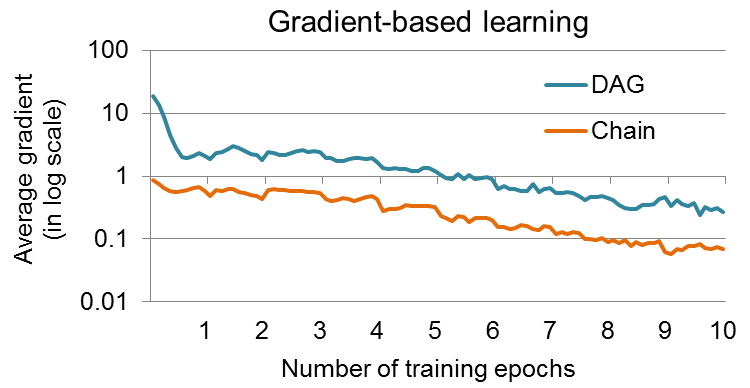
\includegraphics[width=.8\columnwidth,clip=true,trim=10mm 10mm 0mm 0mm]{fig/fig_grad.png}\\
{\footnotesize Number of training epochs}
\caption{The average gradient Layer-1 Conv. during training, plotting in log-scale. Gradients in DAG are consistently 10X larger, implying that they receive a stronger supervised signal from the target label during gradient-based learning.}
\label{fig:grad}
\end{figure}


\section{Discussions\label{sec:ana}}

\subsection{Off-the-shelf DAG}

We first point out an interesting instantiation of our model, linking back to the analysis in Section~\ref{sec:motivation}. We could switch the softmax loss to hinge loss and freeze the back-prop at the FC layer. In this way, we prevent altering the chain-part of our model and only allow training on the augmented part our model, \ie, we learn an linear combination of the FC layers represents multi-scale ReLU activations. Thus, this is equivalent of training a SVM classifier based on the concatenation of the average-pooled activations at all ReLUs. As a result, we could extract multi-scale features using pre-trained CNN models such as the ones in~\cite{AlexNet, veryDeep} and use off-the-shelf SVM solver such as~\cite{liblinear} to train our DAG-CNN model.

%-------------------------------------------------------------------------
%-------------------------------------------------------------------------
\section{Experimental Results\label{sec:exp}}

In this section, we conduct experiments on benchmark datasets, SUN397~\cite{SUN397}, MIT67~\cite{MIT67}, and Scene15~\cite{Scene15}. In absolute terms, we have achieved the best performance ever reported on all three benchmarks. 

\subsection{Experiment Setup}

We should first stress that our DAG model is applied to the ReLU layers selected based on MIT67 dataset, as shown in Fig.~\ref{fig:forward_select}. The learned structure for both Caffe and Deep19 is then used for all the experiments in this Section, demonstrating the data-independence of our approach. We show results of two DAG-structure variants, namely Deep19-DAG and Caffe-DAG in this paper. We have observed similar behavior of other variations.

We follow the standard image pre-processing steps in the literature~\cite{AlexNet,Caffe,veryDeep}. Since both Caffe~\cite{Caffe} and Deep19 models~\cite{veryDeep} have a fixed input size of $224\times 224$, we first resize the image such that the smaller side matches $224$, and then crop an $224\times 224$ patch from the center. The mean RGB value of each model learned on ImageNet~\cite{ImageNet} is then subtracted.  

We show results of using our DAG-structure model for feature extraction. Thus, the output of all the average-pooled ReLU activations are concatenated as our multi-scale representation. For a fair comparison, we compare the multi-scale feature to the best performing single-scale feature. All features are $l2$-normalized. Then the off-the-shelf linear SVM solver~\cite{liblinear} is used to train 67-way one-vs-all classifiers with no parameter tuning.


%-------------------------------------------------------------------------
\subsection{SUN397}

SUN397~\cite{SUN397} is a large scene recognition dataset with 397 categories, each of which includes more than 100 images. The total number of images exceeds 100k. The average classification accuracy is usually report from a 10-fold cross validation. The split file is provided in~\cite{SUN397} with 50 images for training and the rest being test for each fold.  


\begin{table}
\begin{center}
\begin{tabular}{|l|c|}
\hline
Approach & Accuracy(\%) \\
\hline
Deep19-DAG & \textbf{55.5} \\
Deep19~\cite{veryDeep} & 51.9 \\
Caffe-DAG & 46.6	\\
Caffe~\cite{Caffe} & 43.5 \\ \hline
MOP-CNN~\cite{Gong14} & 52.0 \\
Places~\cite{zhoulearning}	& 54.3	\\
DeCaf~\cite{DeCaf} & 40.9	\\
FV~\cite{FV} & 47.2 \\
Baseline~\cite{SUN397} & 38.0 \\
\hline
\end{tabular}
\end{center}
\caption{Classification results on SUN397}
\label{table:SUN397}
\end{table}

We observe that features from our DAG-CNN model always out-perform the single-scale feature on both 
<Achieves best performance>
<talk about Places, using different data -> model structure and better domain specific data are both important>


%-------------------------------------------------------------------------
\subsection{MIT67}

MIT67 refers to the MIT Indoor~\cite{MIT67} scene classification for 67 categories. Indoor scenes depends on highly variable features to describe them. There are cases that can be well characterized by high-level spatial geometry (\eg church and cloister) and low-level textures (\eg wine celler and library). Our multi-scale model is designed to encode feature at all levels, and thus, enable us to learn both high- and low-level statistics of scene categories. The training/test split is made available and there are 80/20 training/test images for each class.

\begin{table}
\begin{center}
\begin{tabular}{|l|c|}
\hline
Approach & Accuracy(\%) \\
\hline
Deep19-DAG & \textbf{76.1} \\
Deep19~\cite{veryDeep} & 70.8 \\
Caffe-DAG & 64.6	\\
Caffe~\cite{Caffe} & 59.5 \\ \hline
MOP-CNN~\cite{Gong14} & 68.9 \\
Places~\cite{zhoulearning}	& 68.2	\\
Mid-level~\cite{mid_level} & 64.0	\\
FV+BoP~\cite{FV_BoP} & 63.2 \\
Disc. Patch~\cite{disc_patch} & 49.4 \\
SPM~\cite{spatial_pyramid} & 34.4	\\
\hline
\end{tabular}
\end{center}
\caption{Classification results on MIT67}
\label{table:MIT67}
\end{table}


%-------------------------------------------------------------------------
\subsection{Scene15}

\begin{table}
\begin{center}
\begin{tabular}{|l|c|}
\hline
Approach & Accuracy(\%) \\
\hline
Deep19-DAG & \textbf{92.4} \\
Deep19~\cite{veryDeep} & 90.8 \\
Caffe-DAG & 89.7	\\
Caffe~\cite{Caffe} & 86.8 \\ \hline
Place~\cite{zhoulearning} & 91.6 \\
CENTRIST~\cite{Wu_pami11} & 84.8	\\
Hybrid~\cite{Bosch_pami08}	& 83.7	\\
Spatial pyramid~\cite{spatial_pyramid} & 81.4 \\
Object bank~\cite{Li_nips10_objectbank}	& 80.9	\\
Reconfigurable model~\cite{Parizi_cvpr12_reconf} & 78.6	\\
Spatial Envelop~\cite{Oliva_ijcv01_envelop} & 74.1 \\
Baseline~\cite{Scene15} & 65.2 \\
\hline
\end{tabular}
\end{center}
\caption{Classification results on Scene15}
\label{table:SUN397}
\end{table}


\subsection{Analysis}

{\bf Per-category analysis}


\begin{figure}[htbp]
\centering
	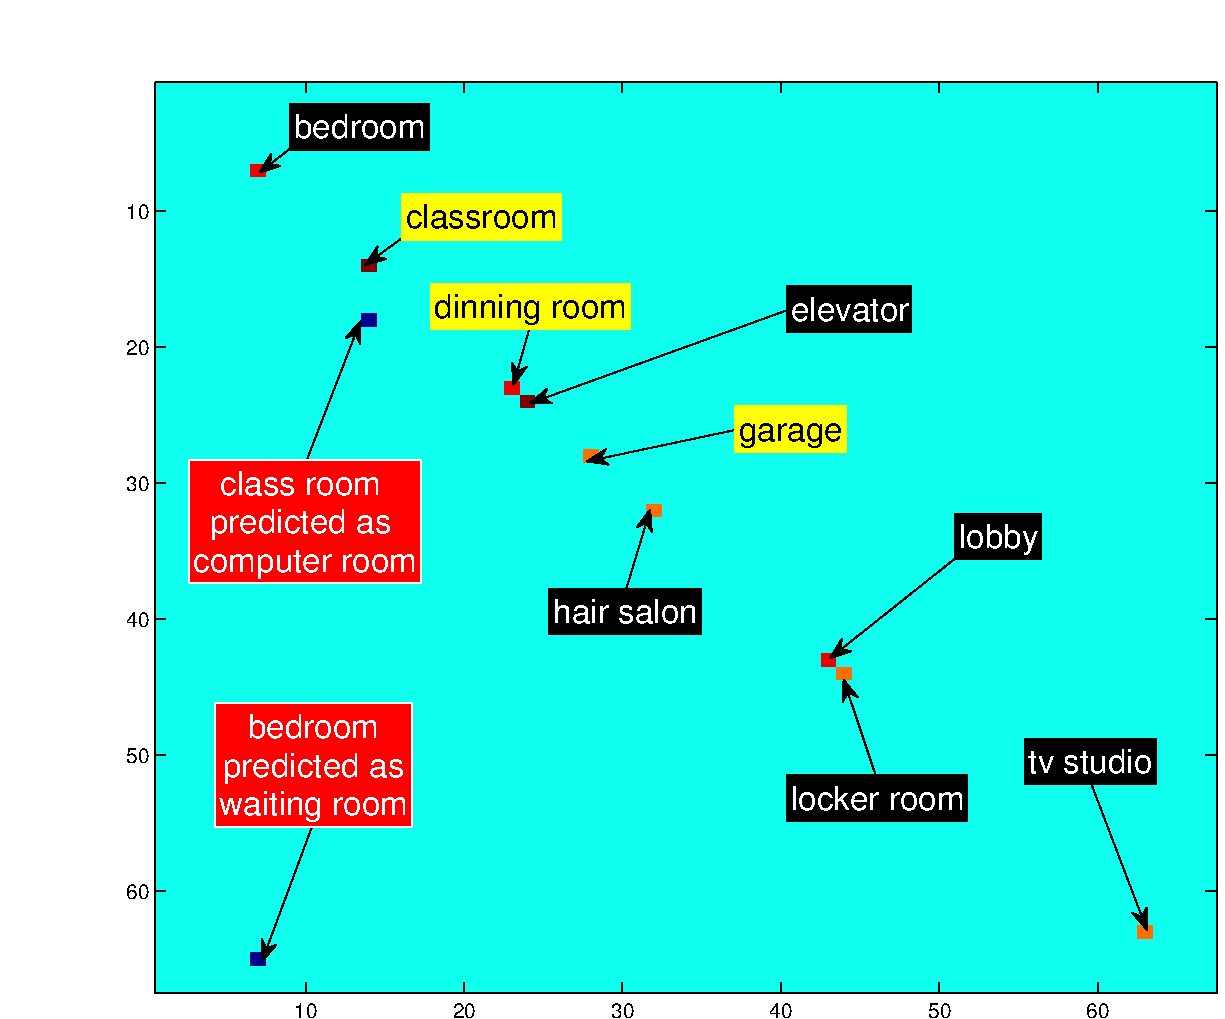
\includegraphics[width=\columnwidth]{fig/fig_conf_diff.pdf}
\caption{The performance improvement of multi-scale over single-scale features on MIT67 in confusion matrix fashion. It is generated by subtracting the the confusion matrix for single-scale from the one for multi-scale. The small differences are ignored. Both \textit{black} and \textit{yellow} label on the diagonal shows the most improved categories, where \textit{black} labels are categories best-classified by high-level features found in Fig.~\ref{fig:best_perf_layer_hist}; similarly, \textit{yellow} label are the ones for mid-level features. \textit{Red} label shows the performance decrease by choosing multi-scale features.}

\label{fig:conf_diff}
\end{figure}


%-------------------------------------------------------------------------
%-------------------------------------------------------------------------
\section{Conclusion}




{\small
\bibliographystyle{ieee}
\bibliography{mobib}
}

\end{document}
